\section{Data creation}

\begin{definition}[\textit{Synthetic data}]
    Synthetic data refers to artificially generated data designed to replicate the characteristics, patterns, and statistical properties of real-world datasets.
\end{definition}
\noindent This type of data can be produced in large volumes and is crafted to closely resemble original datasets, often making it indistinguishable from real data. 
Unlike actual observations, synthetic data does not contain any real-world instances but instead mimics the structure, trends, and relationships found in authentic datasets.

The primary goal of synthetic data generation is to address scenarios where real data is scarce, insufficient, or inaccessible, particularly when privacy concerns limit access to sensitive information. 
Synthetic data can either supplement or replace real-world data, especially in cases where using real data is impractical or restricted. 
The key benefits include handling missing data, mitigating bias, balancing class distributions, enabling secure data sharing, and reducing costs.

\paragraph*{Simulation}
Synthetic data leverages the underlying mechanisms that govern real-world phenomena, allowing for the exploration of new or rare conditions. 
It facilitates the simulation of extreme or uncommon scenarios, which are difficult to observe in real-world settings.

\subsection{Data synthetization}
The concept of data synthesis dates back to 1928 with the advent of sample bootstrapping techniques and has evolved significantly over time.

\begin{chronology}[1]{2010}{2025}{0.9\textwidth}
    \event{2013}{Generative Adversarial Networks}
    \event{2018}{Transformer}
    \event{2022}{ChatGPT 4}
\end{chronology}

Key methods for synthesizing data include:
\begin{itemize}
    \item \textit{Generative Adversarial Networks} (GAN): a Neural Network architecture comprising two components (a generator and a discriminator) that collaborate to produce realistic synthetic data.
    \item \textit{Variational Autoencoder}: models that compress data into a latent space and then reconstruct it, enabling the generation of new samples that closely resemble the original dataset.
\end{itemize}
\noindent These techniques can be applied across diverse domains, including tabular data, text generation, relational databases, time series, 3D modeling, and computer vision.

\paragraph*{Applications}
Synthetic data frameworks are utilized in various use cases:
\begin{itemize}
    \item \textit{Data monetization}: enables secure data sharing and monetization, fostering innovation and competitiveness among businesses of all sizes.
        Companies with valuable but sensitive data often struggle to share it due to privacy regulations like GDPR. 
        Synthetic data allows them to share insights without compromising privacy.
    \item \textit{Fraud detection}: creates balanced datasets to enhance fraud detection models, automates the identification of fake IDs, and removes sensitive customer information from the process.
        Detecting counterfeit IDs used for fraudulent activities is challenging due to privacy concerns and limited access to such documents. 
        Synthetic data helps augment datasets and improve model accuracy.
    \item \textit{Data masking for development}: facilitates the generation of large quantities of data for testing and development, ensuring reproducible scenarios and customizable data for specific needs.
        Sensitive data cannot typically be moved to non-production environments, and random or masked data often lacks realism.
        A synthetic data model trained on production data can replicate sensitive information while preserving privacy.
\end{itemize}
\noindent According to Gartner, by 2030, synthetic data will surpass real data as the primary input for Artificial Intelligence (AI) models.

\paragraph*{Challenges}
Despite its potential, synthetic data faces several challenges:
\begin{itemize}
    \item \textit{Representativeness}: ensuring that synthetic data accurately reflects the statistical properties and complexity of real-world data is a significant hurdle.
        The generated data must capture the diversity and intricacies of actual scenarios to remain useful.
    \item \textit{Validation}: validating synthetic data is critical to ensure that models trained on it generalize effectively to real-world applications. 
        This involves confirming that the synthetic data faithfully represents underlying patterns and relationships.
    \item \textit{Bias and fairness}: the process of generating synthetic data must avoid introducing or amplifying biases, which could lead to unfair or misleading outcomes.
    \item \textit{Transparency}: maintaining transparency in the creation and use of synthetic data is essential. 
        Understanding its origins, characteristics, and limitations ensures responsible and ethical application.
\end{itemize}

\subsection{Generative Artificial Intelligence}
\begin{definition}[\textit{Generative Artificial Intelligence}]
    Generative AI refers to a specialized branch of Artificial Intelligence focused on developing systems capable of producing new data samples that closely resemble the training dataset.
\end{definition}
\noindent Unlike discriminative models, which classify input data into predefined categories or make predictions, generative models aim to understand the underlying structure and distribution of the data. 
By capturing these patterns, generative AI can create novel instances that reflect the characteristics of the original dataset.
In essence, generative AI mimics human-like creativity by learning from examples and producing contextually relevant content across various domains.

\paragraph*{Applications}
Generative AI has a broad range of applications across multiple domains, including:
\begin{itemize}
    \item \textit{Image Generation and Editing}: techniques such as GANs are widely used to generate realistic images. 
        They are also effective for tasks like style transfer, colorization, and image-to-image translation.
    \item \textit{Text Generation and Summarization}: language models can produce coherent and contextually relevant text, making them valuable for tasks like summarization and content creation.
    \item \textit{Content Creation and Augmentation}: generative AI can create entirely new forms of content. 
        Additionally, these models can enhance existing content by generating variations or filling in missing parts.
    \item \textit{Data Synthesis and Simulation}: generative models can create synthetic data that closely resembles real-world data, making them useful for data augmentation, training Machine Learning models, and simulating realistic scenarios. 
\end{itemize}

\begin{definition}[\textit{Large Language Models}]
    A Large Language Model (LLM) is a type of Artificial Intelligence designed to understand and generate human-like text based on the input it receives.
\end{definition}
\noindent These models are trained on vast amounts of text data, typically sourced from the internet or other extensive corpora, enabling them to learn the intricate patterns and structures of human language. 
LLMs are built using deep learning architectures, often based on transformer architectures, which consist of multiple layers of neural networks. 
These layers process input text hierarchically, capturing both local and global dependencies within the text. The result is a model capable of producing highly coherent and contextually relevant text.

Once trained, LLMs can perform a wide variety of natural language processing tasks, including text generation, completion, translation, summarization, and question answering.
Their ability to generate fluent and contextually appropriate text has made them indispensable in applications such as virtual assistants, content creation, and more.

\subsubsection{Prompt engineering}
\begin{definition}[\textit{Prompt engineering}]
    Prompt engineering is the practice of designing and crafting prompts or inputs to interact with language models or AI systems in order to achieve specific, desired outputs.
\end{definition}
\noindent The goal of prompt engineering is to optimize how questions or requests are framed to ensure the AI generates accurate, useful, and relevant responses. 
Key strategies for effective prompting include being clear and specific, providing relevant context, asking open-ended questions, using important keywords, avoiding ambiguity, engaging in conversation, offering feedback, and experimenting with different approaches.

\subsubsection{Multimodal generative AI}
Multimodal generative AI refers to systems capable of creating content across multiple modalities. 
These advanced AI systems leverage machine learning techniques to process and generate content from various types of data.

Unlike traditional generative models that focus on a single modality, 
multimodal models can handle multiple data types simultaneously, enabling richer and more comprehensive content generation. 
These models understand the relationships between different forms of data, resulting in more contextually relevant and dynamic outputs.

\paragraph*{Training}
Training multimodal AI models requires large, diverse datasets that include paired examples of different data types.
 These datasets help the model learn the correlations and connections between various modalities, enhancing its ability to generate accurate and coherent content across different media formats.

\subsubsection{Enterprise applications}
\begin{definition}[\textit{Retrieval Augmented Generation}]
    Retrieval Augmented Generation (RAG) is a technique in natural language processing that combines retrieval-based methods with generative models to improve the quality and relevance of generated text.
\end{definition}
\noindent In RAG, a retriever component searches a large database or text corpus to find information relevant to the input query or context. 
This retrieved information is then used to enhance the generative model's output, producing responses that are more accurate, coherent, and contextually relevant. 
With RAG, enterprise data can be leveraged to enrich prompts and improve performance.

\paragraph*{Architecture}
Enterprise architectures incorporating generative AI typically include the following components:
\begin{itemize}
    \item \textit{Vectorial database layer}: a storage layer that organizes data in a format easily understood by large language models.
    \item \textit{Feedback}: a mechanism to collect feedback and contextual information, enabling continuous improvement and evolution of the model.
    \item \textit{RAG agent}: the core component responsible for managing inputs and outputs, integrating retrieval and generation processes.
    \item \textit{Guard rail}: a safeguard to prevent model leakage or malicious attacks, ensuring the quality and security of outputs.
        However, limiting the LLM's capabilities may degrade performance and increase latency, as all inputs and outputs must be checked.
    \item \textit{LLM gateway and catalog}: responsible for routing prompts to the most suitable large language model for processing.
\end{itemize}

\begin{figure}[H]
    \centering
    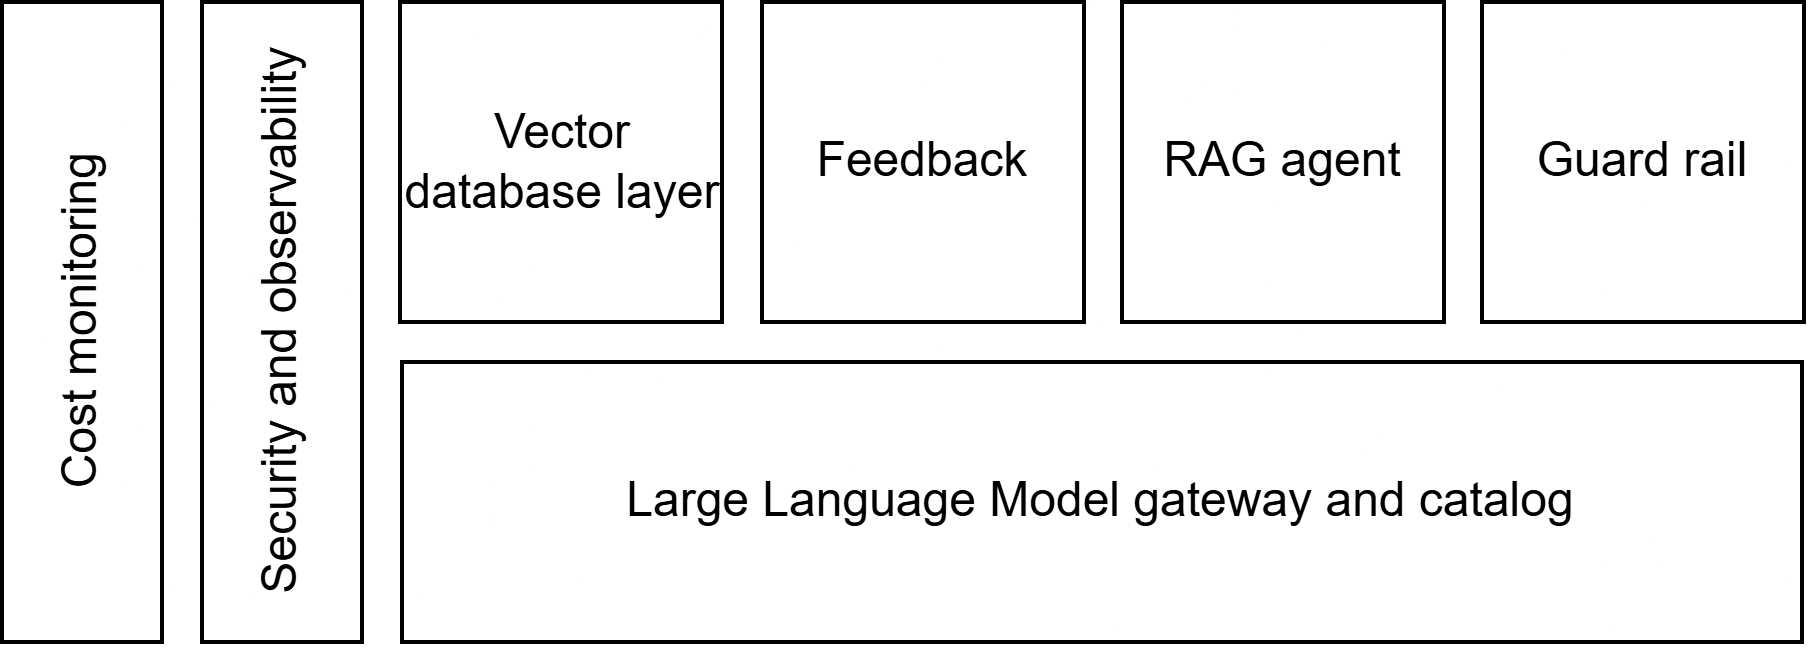
\includegraphics[width=0.75\linewidth]{images/bis14.png}
    \caption{Architecture}
\end{figure}

\subsection{Explainable Artificial Intelligence}
Explainable Artificial Intelligence (XAI) is a research field dedicated to developing techniques that interpret machine learning models and explain their predictions in terms understandable to humans. 
As Machine Learning models become more accurate and sophisticated, their complexity often increases, turning them into black boxes where the decision-making process is opaque and difficult to comprehend. 
This lack of transparency raises concerns about the trustworthiness, fairness, and accountability of AI systems.

The growing reliance on AI in critical domains—such as healthcare, finance, and law.
When AI systems make decisions that impact individuals or society, it is essential to understand the rationale behind those decisions. 
XAI addresses these challenges by ensuring that AI models are not only accurate but also interpretable, fair, and free from biases.

\subsubsection{Post-hoc methods}
Post-hoc explainability methods aim to make predictions from existing machine learning models interpretable without altering the model itself. 
These methods can be categorized as follows:
\begin{itemize}
    \item \textit{Model specific}: these methods leverage the internal structure and learning algorithm of a specific model to provide explanations tailored to its architecture.
    \item \textit{Model agnostic}: these methods analyze the relationship between model inputs and predictions in a generalizable way, making them applicable to any type of model.
    \item \textit{Global}: these methods provide an overarching explanation of the model's behavior across the entire dataset, offering insights into how the model operates as a whole.
    \item \textit{Local}: these methods focus on explaining individual predictions or subsets of data, providing detailed insights into specific instances.
\end{itemize}
\noindent Common post-hoc XAI approaches include feature importance, surrogate models, rule-based models, and saliency maps. 

\subsubsection{Reponsible AI}
Responsible AI is a broader framework that encompasses various sub-disciplines aimed at ensuring AI systems are developed and deployed ethically and responsibly. 
These sub-disciplines include: explainable AI, human-centered AI, compliance, ethical AI, secure AI, and interpretable AI. 